\documentclass[12pt]{article}
\usepackage[utf8]{inputenc}
\usepackage{listings}
\usepackage{c/style} % include custom style for C
\usepackage{plain/plain_style} % include custom style for plain text
\usepackage{amsmath}
\usepackage{graphicx}

\title{Generazione automa caratteristico parsing bottom-up LR(0) }
\author{
        Sandri Fabrizio \\ \\        
        Dipartimento di Ingegneria e Scienza dell'Informazione\\
        Università di Trento
}

\date{\today}


\begin{document}
\maketitle

\section{Introduzione}
In questo report si vuole analizzare ed implementare la procedura di generazione di un automa caratteristico per il parsing bottom-up di tipo LR(0). Fra i vari tipi di parsing visti a lezione il parsing LR(0) è un tipo di parsing per cui si legge l'input da sinistra a destra e si produce una derivazione di tipo rightmost a partire dalla grammatica data in input.

\paragraph{Il problema:} 
il primo step del parsing bottom-up è quello di generare un automa caratteristico a partire dalla grammatica letta in input per poi andare a formare una tabella di parsing. In questo report ci focalizzeremo solamente sulla parte di generazione dell'automa caratteristico.

\section{Definizioni}
L'automa caratteristico è formato da un insieme di stati interconnessi da una funzione di transizione $\tau$ definita su coppie di stati. 
Ogni stato contiene degli LR(0)-items : alcuni di questi item faranno parte del kernel, mentre altri fanno parte della closure del kernel.\\

La tecnica di costruzione dell'automa caratteristico è incrementale: andiamo a popolare un set di stati definendo mano a mano la funzione di transizione, fino a saturazione. Nel dettaglio l'algoritmo di generazione dell'automa seguirà i seguenti step:
\begin{description}
\item[-] Lettura della grammatica fornita in input dall'utente ed estrazione delle produzioni con rimozione di eventuali spazi dalla produzione;
\item[-] Aggiunta di una fresh production alla grammatica facendo attenzione ad aggiungere un simbolo nuovo in modo da evitare conflitti;
\item[-] Creazione e aggiunta dello stato iniziale all'automa caratteristico (stato 0), costituito da un singolo Item LR(0), quello della fresh production;
\item[-] Calcolo della closure dell'Item contenuto nello stato iniziale con aggiunta delle nuove transizioni verso nuovi stati. In questo step bisognerà fare attenzione a non aggiungere un nuovo stato se il kernel è identico a quello di uno stato già aggiunto in precedenza: bisognerà quindi ricercare nell'automa se esiste uno stato con lo stesso kernel;
\item[-] Per ogni nuovo stato creato si calcola il kernel e lo si aggiunge agli items dello stato stesso;
\item[-] A partire dal kernel del nuovo stato si calcola la closure e si aggiungono le nuove transizioni verso i nuovi stati;
\item[-] Si eseguono gli ultimi due punti fino a saturazione, ovvero finché ci sono nuovi stati, ovvero stati non marcati nell'automa caratteristico;
\item[-] Giunti al termine si stampano a video le transizioni e tutte le informazioni sui singoli stati dell'automa.
\end{description}


\section{Strutture dati}
Per implementare l'automa caratteristico dato in output dal programma e la grammatica fornita in input si è cercato di seguire uno stile di programmazione il più astratto e intuitivo possibile, in modo da rendere la lettura del codice di facile comprensione. In particolare il linguaggio C non offrendo delle strutture dati pre fabbricate ci ha obbligati a definirne alcune, sfruttando la keyword $struct$.\\

Analizzeremo nei prossimi paragrafi le decisioni implementative prese per realizzare le varie parti necessarie alla costruzione di un automa caratteristico. Riportiamo in breve di quali importanti strutture dati ci avvaleremo durante la trattazione:
\begin{enumerate}
\item Produzione
\item Grammatica
\item Item LR(0)
\item Funzione di transizione
\item Stato dell'automa caratteristico
\item Automa caratteristico
\end{enumerate}

\subsection{Produzione}
La produzione è una struttura dati di base su cui si basa la grammatica, essa è una struttura minimale composta da 3 parti:
\begin{list}{-}{}
\item char driver : il driver della produzione ;
\item char[ ] body : stringa contenente il body della produzione ;
\item int production\_id : valore intero utilizzato per controllare in maniera efficiente se le produzioni memorizzate in due item distinti sono uguali. Se driver e body di due item distinti avranno lo stesso $production\_id$ vorrà dire che la produzione memorizzata nell'item sarà identica e meno della posizione del marker che può essere differente.
\end{list}

Riportiamo ora il codice utilizzato per rappresentare una produzione.
\lstinputlisting[language=C,style=c]{c/fragments/production.c}

\subsection{Grammatica}
Il primo step nella procedura di generazione dell'automa caratteristico è quello di leggere la grammatica fornita in input dall'utente e memorizzarla. Vista la definizione di $production$ fornita in precedenza definiamo la grammatica come un array di produzioni.\\

Ogni nuova produzione sarà inserita nella grammatica sfruttando la funzione $addProduction()$ che si occuperà di rimuovere gli spazi e dividere le produzioni multi-definite, ovvero le produzioni con lo stesso driver ma con body differente unite dall'operatore $|$ e scritte sulla stessa riga . \\

Riportiamo qui sotto il codice utilizzato per rappresentare la grammatica.
\lstinputlisting[language=C,style=c]{c/fragments/grammar.c}



\subsection{Item LR(0)}
Gli stati dell'automa caratteristico saranno formati da Item LR(0), ovvero Item associati ad una singola produzione e ad un marker
$$
A \to \alpha\cdot\beta
$$ 
Dove il simbolo $\cdot$ indica la posizione del marker all'interno del body della produzione. \\

A livello implementativo un modo efficiente per implementare un Item LR(0) è quello di utilizzare una struct contenente le seguenti informazioni:
\begin{list}{-}{}
\item production prod : la produzione associata all'item e definita sfruttando la definizione di produzione vista in precedenza;
\item int marker\_position : un valore intero rappresentante la posizione del marker all'interno dell'item;
\item bool isKernelProduction : settato a true per indicare che un Item fa parte del Kernel di uno stato.
\end{list}

Riportiamo ora il codice utilizzato per rappresentare gli Item LR(0).
\lstinputlisting[language=C,style=c]{c/fragments/lr0_item.c}

\subsection{Funzione di transizione}\label{tau}
La funzione di transizione associa ad una coppia (stato, letterale) un altro stato. Se diciamo S gli stati dell'automa caratteristico e V il vocabolario della grammatica considerata allora definiamo formalmente la funzione di transizione come
$$
\tau \colon (S, V) \to S
$$

Per poter implementare questa funzione nel modo più semplice ed efficiente possibile adottiamo una struttura avente 3 attributi:
\begin{list}{-}{}
\item int from : lo stato origine della transizione
\item int to : lo stato destinazione della transizione
\item char by : un letterale equivalente al valore che leggerò nell'input buffer. In altre parole questo sarà il letterale che etichetterà l'arco di transizione 
\end{list}

Riportiamo il codice della struttura associata alla funzione di transizione.
\lstinputlisting[language=C,style=c]{c/fragments/transition.c}



\subsection{Stato dell'automa caratteristico}
Ogni stato dell'automa caratteristico sarà definito da un identificativo numerico: la posizione nell'array $automa$ definito nella prossima sezione "Automa caratteristico". Descriveremo il singolo stato attraverso i seguenti attributi:
\begin{list}{-}{}
\item lr0\_item items[50] : dalla definizione sappiamo che ogni stato dell'automa caratteristico sarà composto da un insieme di LR(0) items, in questo caso definito tramite un array. Alcuni di questi items inoltre faranno parte del kernel dello stato.
\item transaction transactions[MAX\_AUTOMA\_STATES\_COUNT] : un insieme di transizioni uscenti dallo stato corrente e dirette nel verso degli altri stati. Anche in questo caso sfruttiamo la definizione di $struct transaction$ definita in precedenza.
\item state\_type type : indica il tipo di stato corrente che può essere uno stato fra i seguenti : $normale$, di $accept$ oppure $finale$.
\item int items\_count : numero totale di items presenti nello stato(compresi quelli facenti parte del kernel)
\item int kernel\_items\_count : numero di items che sono parte del kernel. Questa variabile è aggiunta al solo scopo di velocizzare la procedura di controllo della presenza di uno stato con lo stesso kernel nell'automa caratteristico. Se due stati hanno numero di items del kernel diverso, sicuramente non potranno essere uguali e quindi si saltano calcoli aggiuntivi.
\item int transaction\_count : numero di transizioni uscenti dallo stato
\end{list}

L'implementazione dello stato dell'automa caratteristico rispecchia esattamente i punti appena visti.
Riportiamo il codice utilizzato per rappresentare lo stato dell'automa.
\lstinputlisting[language=C,style=c]{c/fragments/automa_state.c}

\subsection{Automa caratteristico}
Siamo giunti all'ultima struttura : l'automa caratteristico per il parsing bottom-up LR(0). Abbiamo tutte le strutture necessarie per definirlo. Rappresenteremo l'automa attraverso un insieme di stati definiti come nel precedente paragrafo.\\

Riportiamo per completezza il codice per definire l'automa
\lstinputlisting[language=C,style=c]{c/fragments/automa.c}

\section{Input e Output}

\subsection{Input}
La procedura di generazione dell'automa caratteristico assume che sia fornita una grammatica in input seguendo una particolari sintassi. Esistono due modi per fornire la grammatica:
\begin{enumerate}
\item Input da parte dell'utente
\item Input da file
\end{enumerate}

Entrambi questi metodi assumono che l'input sia fornito in un formato standard come specificato nel prossimo paragrafo.

\subsubsection{Formato input}\label{sec:inputformat}
La grammatica fornita dall'utente dovrà rispettare le seguenti regole sintattiche:
\begin{enumerate}
\item Ogni produzione dovrà essere della forma \texttt{A -> $\alpha$} dove A è un non terminale e $\alpha$ è un insieme di simboli terminali e non terminali. 
\item driver e body delle produzioni dovranno essere separati da due caratteri "trattino" e "maggiore" formando il simbolo \texttt{->} 
\item ogni letterale della grammatica, terminale o non terminale che sia, sarà rappresentato da un singolo carattere. Ad esempio se si volesse rappresentare il terminale $digit$ saremo costretti a utilizzare un solo carattere $d$. La sequenza $digit$ altrimenti verrebbe interpretata come 5 terminali
\item non facendo parte dello standard ascii supportato dal linguaggio C, il carattere $\epsilon$ verrà rappresentato dal carattere $\sim$.
La produzione $A \to \epsilon$ verrà quindi rappresentata come \texttt{A -> $\sim$}
\item ogni spazio inserito nelle produzioni verrà rimosso in modo da evitare che il carattere di spaziatura sia considerato un terminale.

\end{enumerate} 

\subsubsection{Input da parte dell'utente}
L'utente eseguirà il programma e dopo aver passato lo start symbol della grammatica come parametro dovrà inserire manualmente ogni singola produzione separata da un carattere "a capo". Per terminare l'inserimento si dovrà semplicemente cliccare il tasto "Enter" dopo aver inserito l'ultima produzione. Ogni produzione dovrà rispettare lo standard specificato della sezione \ref{sec:inputformat}.\\

\paragraph{Esempio}
Supponiamo di avere in input la seguente grammatica avente come start symbol $S$ e di voler generare l'automa caratteristico associato.
\begin{align*}
    S \to aABe \\
	A \to Abc \mid b \\
	B \to d 
\end{align*}

L'utente eseguirà il programma compilato passando lo start symbol S e le produzioni una per volta come nel seguente frammento estratto dalla shell
\lstinputlisting[language=C,style=c]{bash_fragments/user_input.bash}


\subsubsection{Input da file}
In alternativa all'input manuale delle produzioni, l'utente potrà specificare un file di input contenente la grammatica utilizzando due metodi diversi:
\begin{enumerate}
\item parametro al programma
\item ridirezione dell'input
\end{enumerate}

Descriviamo entrambe le alternative
\paragraph{1. Parametro del programma} L'utente fornisce un secondo ulteriore parametro al programma contenente la posizione del file di input. 

\subparagraph{Esempio}
Supponiamo di avere in input la stessa grammatica dell'esempio precedente per l'input da parte dell'utente. In questo caso però assumiamo che la grammatica sia memorizzata in un file di testo nella cartella "test\_grammars" chiamato "grammar5.txt"\\

L'utente eseguirà il programma compilato passando lo start symbol S e la posizione del file come riportato nell'estratto di codice qui sotto
\lstinputlisting[language=C,style=c]{bash_fragments/file_input_parameter.bash}

\paragraph{2. Ridirezione dell'input}L'utente utilizzando l'operatore di ridirezione $>$ fornito dal linguaggio bash su GNU/Linux ridireziona il contenuto del file contenente la grammatica allo standard input del programma. 

\subparagraph{Esempio}
Anche in questo caso supponiamo di avere in input la grammatica "grammar5.txt" dell'esempio precedente. L'utente eseguirà il programma compilato passando lo start symbol S e ridezionerà il contenuto del file della grammatica al programma come nel seguente frammento di codice estratto dalla shell
\lstinputlisting[language=C,style=c]{bash_fragments/file_input.bash}


\subsection{Output}\label{output}
In output il programma ritornerà a video l'automa caratteristico con tutte le informazioni ad esso annesse. Descriviamo nei prossimi paragrafi le informazioni restituite in output dall'esecuzione del programma sulla seguente grammatica: 
\begin{align*}
    S \to aABe \\
	A \to Abc \mid b \\
	B \to d 
\end{align*}

\lstinputlisting[style=plain]{plain/output1.txt}

Come si evince dal listato sopra, l'output sarà diviso in 3 parti:

\begin{enumerate}
\item Grammatica: la prima parte conterrà la grammatica letta in input con aggiunta la fresh production generata a partire dal nuovo fresh symbol(specificato a linea 1) e dallo start symbol passato come parametro.

\paragraph{NOTA:}il fresh symbol viene calcolato in automatico a partire da una lista di non terminali (lettere dell'alfabeto da A a Z, solitamente la scelta ricade sulla lettera K in quanto le lettere A, B e C sono spesso presenti nelle grammatiche che abbiamo visto, riducendo il numero di tentativi necessari per cercare un nuovo non terminale).

\item Transizioni : la seconda parte contiene una lista di transizioni dai vari stati, rispettando la definizione di funzione di transizione vista nella sezione \ref{tau}.
\paragraph{Esempio: } \texttt{Tau(0,S) = 1} indica una transizione dallo stato 0 allo stato 1 tramite il non terminale S.

\item Items degli stati: per ogni stato dell'automa caratteristico vengono stampati il valore identificativo dello stato, il tipo di stato e i rispettivi items che lo compongono. \\

Il tipo di stato può assumere un valore fra i seguenti:
\begin{list}{-}{}
\item finale : sono marcati come finali tutti gli stati che contengono almeno un reducing item;
\item accept : esiste un solo stato di accept ed è lo stato contenente il reducing item per la fresh production;
\item normale : qualsiasi altro stato che non contiene alcun reducing item.
\end{list}

\end{enumerate}


\section{Testing}
Per testare l'effettivo funzionamento dell'algoritmo si è deciso di procedere eseguendo dei test di difficoltà incrementale, partendo da grammatiche semplici composte da poche produzioni fino ad arrivare a grammatiche costituite da più produzioni con lo stesso driver separate da $\mid$ e con l'aggiunta di produzioni con body uguale a $\epsilon$.\\

Nella directory \texttt{test\_grammars} sono presenti alcune grammatiche d'esempio viste a lezione. Queste ultime sono state testate una ad una producendo dei risultati corretti e in linea con gli automi caratteristici generati a lezione, a meno dell'ordinamento di assegnazione dei nomi agli stati. Riportiamo in seguito il risultato dell'esecuzione su alcune di esse.


\subsection{Grammatica 1}
La prima grammatica che testeremo è una grammatica molto semplice costituita da 4 produzioni. In questo caso vediamo in azione le potenzialità dell'operatore di unione $\mid$ il quale ci permette di scrivere più produzioni con lo stesso driver sulla stessa riga. \\

Riportiamo per completezza la grammatica in questione:
\lstinputlisting[style=plain]{../test-grammars/grammar1.txt}

L'esecuzione del programma su questa grammatica genera in output l'automa caratteristico descritto secondo il formato specificato nella sezione dedicata all'interpretazione dell'output(Sezione \ref{output}).
\lstinputlisting[style=plain]{plain/output1.txt}
\begin{figure}[h]
  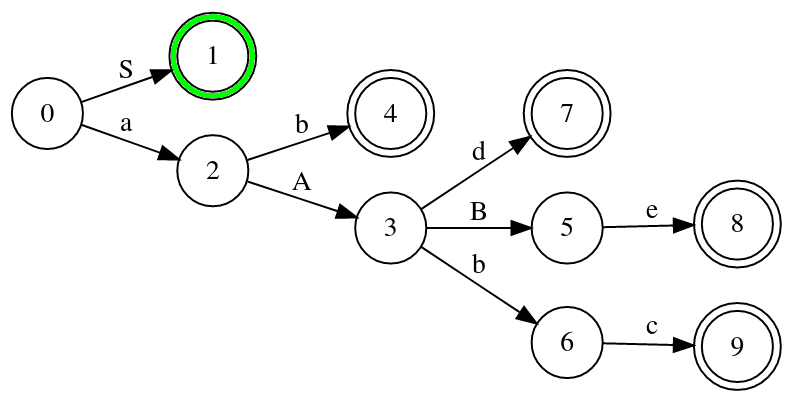
\includegraphics[height=6cm, keepaspectratio]{assets/automa1.png}
  \caption{Automa caratteristico per la Grammatica in questione}
  \label{fig:automa1}
\end{figure}

\subsection{Grammatica 2}
La seconda grammatica descrive della banali operazioni di somma e moltiplicazione. Riportiamo la grammatica in questione:
\lstinputlisting[style=plain]{../test-grammars/grammar2.txt}

L'esecuzione del programma su questa grammatica genera in output l'automa caratteristico descritto secondo il formato specificato nella sezione dedicata all'interpretazione dell'output(Sezione \ref{output}).
\lstinputlisting[style=plain]{plain/output2.txt}
\begin{figure}[h]
  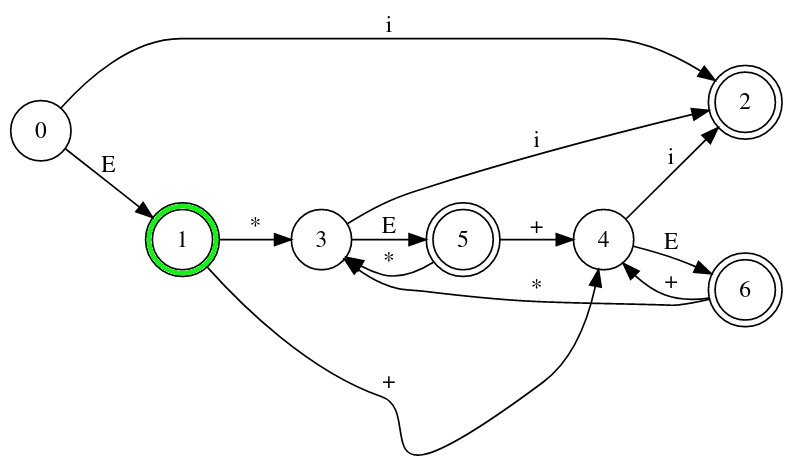
\includegraphics[height=9cm, keepaspectratio]{assets/automa2.png}
  \caption{Automa caratteristico per la Grammatica in questione}
  \label{fig:automa1}
\end{figure}


\subsection{Grammatica 3}
La terza grammatica è simile alla grammatica 3 ma con l'aggiunta delle parentesi e un operatore di sottrazione al posto di quello di moltiplicazione. Sarà ora possibile combinare espressioni multiple e separarle utilizzando delle parentesizzazioni. Riportiamo per completezza la grammatica in questione:
\lstinputlisting[style=plain]{../test-grammars/grammar3.txt}

L'esecuzione del programma su questa grammatica genera in output l'automa caratteristico descritto nel seguente listato
\lstinputlisting[style=plain]{plain/output3.txt}
\begin{figure}[h]
  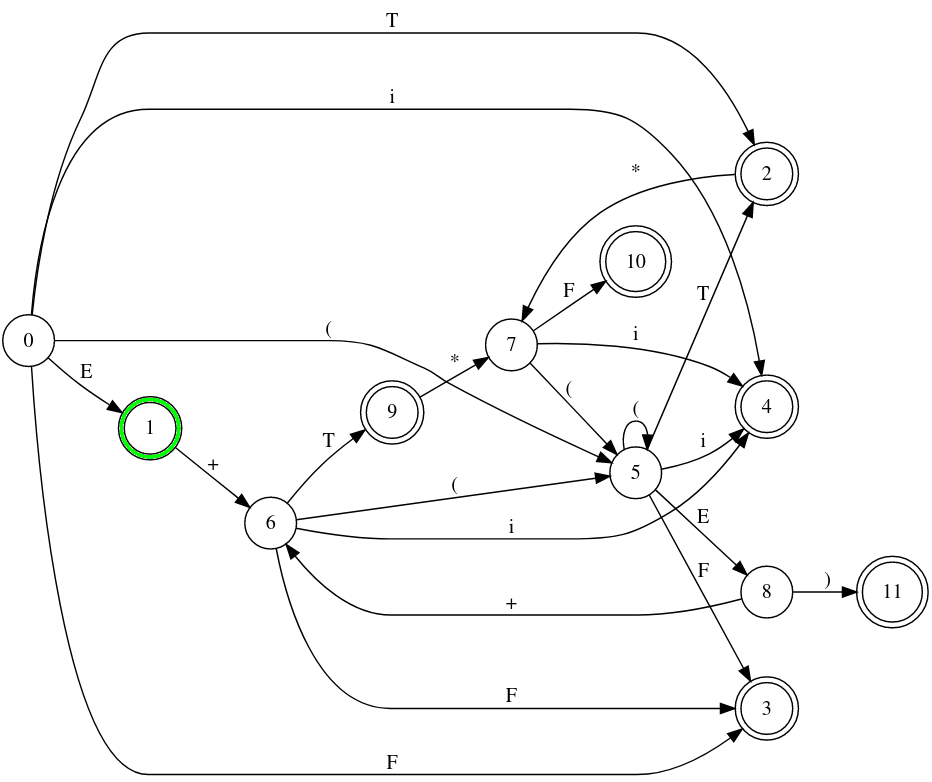
\includegraphics[height=13cm, keepaspectratio]{assets/automa3.png}
  \caption{Automa caratteristico per la Grammatica in questione}
  \label{fig:automa1}
\end{figure}

\subsection{Grammatica 6}
Riportiamo l'output della Grammatica 6, tralasciando la grammatica 4 e e la grammatica dei puntatori 5 per non appesantire troppo il report: il lettore può eseguire in autonomia il programma per la generazione dell'automa caratteristico applicato alle grammatiche suddette.\\

La grammatica 6 viene riportata in questo report in quanto contiene delle $\epsilon$-produzioni e come specificato nelle sezione \ref{sec:inputformat} dedicata al Formato dell'Input le $\epsilon$-produzioni dovranno essere scritte utilizzando il simbolo 
$\sim$. \\

Riportiamo la grammatica in questione:
\lstinputlisting[style=plain]{../test-grammars/grammar6.txt}

Come possiamo vedere le produzioni 
\begin{align*}
\texttt{A -> $\epsilon$} \\
\texttt{B -> $\epsilon$}
\end{align*}
sono state riscritte rispettivamente come 
\begin{align*}
\texttt{A -> $\sim$} \\
\texttt{B -> $\sim$}
\end{align*}

L'esecuzione genererà l'output del seguente listato
\lstinputlisting[style=plain]{plain/output6.txt}
\begin{figure}[h]
  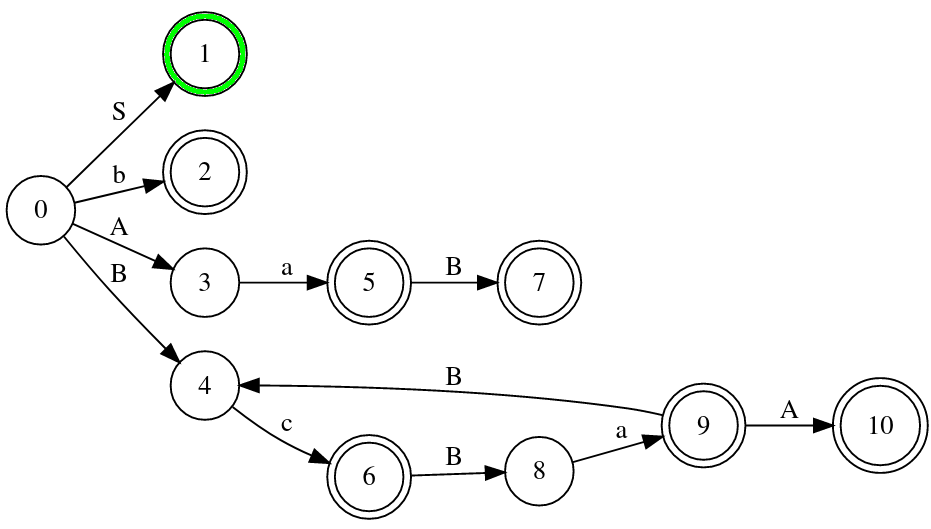
\includegraphics[height=7cm, keepaspectratio]{assets/automa6.png}
  \caption{Automa caratteristico per la Grammatica in questione}
  \label{fig:automa1}
\end{figure}

\end{document}